\section{Experimental Method and Locked Simulator Evidence}
\label{sec:locked-evidence}

We evaluate recovery after subscriber-pod scale-out using 20,000 subscriptions,
ten persistent connections, and 775 million queued events. The primary
comparison measures the use of added pod capacity with guarded-greedy and
DQL-guided migration against retaining the initial connection placement. Supporting studies examine
multi-objective control, action selection, and adverse probe promotion.

\subsection{Recovery After Subscriber-Pod Scale-Out}
\label{sec:scaleout-recovery}

The primary recovery experiment models the capacity increase from one
subscriber pod to four. Ten persistent TCP connections are established on the
original pod, carrying 20,000 subscriptions. At the measurement boundary,
three additional ready pods provide processing capacity, while the ten
established connections retain their original endpoints. The comparison
therefore measures how effectively the client uses the added capacity through
probe promotion and subscription reassociation.

Four equal subscription groups begin with 100,000, 50,000, 5,000, and zero
queued events per subscription, respectively. The initial backlog is
$B(0)=775{,}000{,}000$ events. Round-robin assignment gives each connection
2,000 subscriptions and 77.5 million queued events. Consequently,
$V^N_u(0)=V^G_u(0)=0$: the initial bottleneck is concentrated pod placement.
This setup isolates whole-connection migration from pre-existing imbalance
between the client's connections.

The model assigns each pod a processing threshold of 100,000 events/s and
the client a base acknowledgement capacity of 250,000 events/s. Its bounded
connection-parallelism factor is three at ten connections. Service is limited
by both client capacity and each connection's share of its pod capacity.
The simulator's pressure-dependent service factor is
$\max\{0.35,1-0.42P_i^{\mathrm{sim}}\}$, where $P_i^{\mathrm{sim}}\in[0,1]$ is the simulator's
clipped load score, distinct from the deployable pressure in
(\ref{eq:pod_pressure}). These numerical rates define the simulator's service
assumptions rather than measured Pod benchmarks. Pressure is sampled before the action
and refreshed after the interval. For the clipped score, this service
multiplier lies in $[0.58,1]$: the model represents pressure-degraded service,
not complete Pod service collapse. Arrival rates and processing rates are
converted to event counts using the declared $\Delta=10$ seconds. The drain
phase introduces no new arrivals and lasts 120 intervals, or 20 minutes.

We compare \emph{Frozen DQL}, \emph{Kubernetes scale-out only}, and
\emph{Scripted probe migration}. All three receive the same capacity increase.
The second policy retains the existing connection assignment. The third
promotes every candidate admitted by the migration guard and evaluates the
framework's deterministic guarded-greedy policy. DQL uses the previously frozen checkpoint
without exploration or training. Adaptive policies can replace at most 12
non-improving probes, and actions have a three-interval cooldown.
The scripted control uses no learned Q-values: it shares the pressure-aware
admission rule and source selection with DQL. We therefore distinguish this
\emph{guarded-greedy} policy from the independent ad-hoc schedules below.
Its mean throughput is 221,260 events/s, compared with 219,762 for DQL. These
are two effective selectors for the shared rebalancing mechanism, not evidence
that Q-learning is necessary to use added capacity. The original registered
primary contrast remains DQL versus unchanged placement; this broader
interpretation does not change that protocol or relabel a post-hoc contrast
as confirmatory. An exploratory paired reanalysis of these same twenty seeds
gives a greedy-minus-DQL mean throughput difference of 1,498 events/s
(pointwise percentile bootstrap 95\% interval [362, 2,852], 10,000 resamples).
This small rate advantage belongs to the greedy policy in this workload;
the mixed-workload study evaluates DQL's separate multi-objective benefit.

For remaining backlog $B(t)$, the primary endpoint is the mean normalized
backlog over the recovery window,
\begin{equation}
 \mathrm{AUC}_B=\frac{1}{T}\sum_{t=1}^{T}
 \frac{B(t-1)+B(t)}{2B(0)},\qquad T=120.
 \label{eq:scaleout-backlog-auc}
\end{equation}
Lower $\mathrm{AUC}_B$ indicates less accumulated queued work. Twenty fresh paired seeds
vary probe placement while holding the workload fixed. We use 10,000 paired
bootstrap resamples and 100,000 sign-randomization draws. The registered
criterion requires the upper 95\% confidence bound of the DQL-minus-baseline
AUC difference to be below zero and the one-sided $p$-value to be below 0.05.
These intervals describe variation caused by probe placement within this model.

\begin{table}[!t]
\centering
\small
\caption{Persistent-connection recovery after scaling from one to four subscriber Pods. Twenty paired seeds each start with 20,000 subscriptions and 775 million queued events on ten TCP connections pinned to Pod~0. Lower backlog measures are better.}
\label{tab:persistent_scaleout_recovery}
\resizebox{\linewidth}{!}{%
\begin{tabular}{lrrrrr}
\toprule
Policy & Backlog AUC & Final backlog (\%) & Throughput (k/s) & Active Pods & Migrations \\
\midrule
\textbf{Frozen DQL} & 0.8376 & 65.97 & 219.8 & 4.00 & 7.75 \\
Kubernetes scale-out only & 0.9551 & 91.02 & 58.0 & 1.00 & 0.00 \\
Scripted probe migration & 0.8359 & 65.74 & 221.3 & 4.00 & 7.75 \\
\midrule
\multicolumn{6}{l}{DQL vs. scale-out only: 12.30\% lower backlog AUC; 278.9\% higher mean throughput.} \\
\bottomrule
\end{tabular}
}
\end{table}


Table~\ref{tab:persistent_scaleout_recovery} shows that DQL raises mean
throughput from 58,000 to 219,762 events/s, a factor of 3.79. It reduces backlog
AUC from 0.95510 to 0.83759, an improvement of 12.30\%. The paired AUC
difference is $-0.117504$ (95\% confidence interval
$[-0.121210,-0.113345]$; one-sided $p\simeq10^{-5}$). DQL leaves 65.97\% of
the initial backlog after 20 minutes, compared with 91.02\% for scale-out only,
or 27.52\% less remaining backlog relative to that baseline. All 20 DQL
episodes use all four pods by the end, with a mean of 7.75 connection
migrations. The baseline retains all ten connections on the original pod.

\begin{figure}[!htbp]
 \centering
 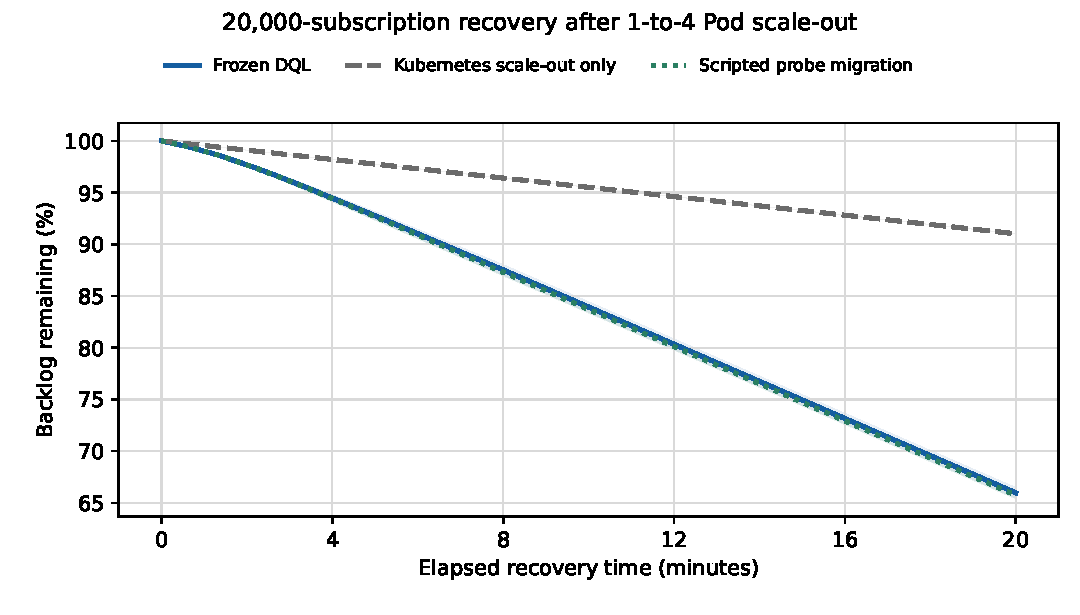
\includegraphics[width=\textwidth]{evidence/persistent-scaleout-recovery-complete/persistent_scaleout_backlog_recovery.pdf}
 \caption{Backlog recovery after adding three subscriber pods. All policies
 start with the same 775-million-event backlog. Curves are means over 20
 paired seeds; shaded bands are descriptive 95\% normal-approximation
 intervals. The area under each normalized curve defines the primary endpoint.}
 \Description{A line chart compares remaining backlog over twenty minutes.
 DQL and scripted probe migration drain substantially more backlog than
 Kubernetes scale-out with the original TCP connection placement.}
 \label{fig:scaleout-backlog-recovery}
\end{figure}

Figure~\ref{fig:scaleout-backlog-recovery} connects the endpoint to the
recovery process. The steeper DQL curve follows successful probe promotions
that place delivery work on additional pods. The nearby scripted-control curve shows that DQL reaches about the same
service capacity as guarded scripted migration. Both improve on the unchanged
placement, establishing the benefit of migration in this workload rather than
a ranking above every controller with the same actions.

Capacity-activation timelines, seed-level violin plots, and independent
ad-hoc timing controls are retained in Section~\suppref{app:scaleout-details} of
the Online Supplementary Material. Those controls do not replace the
pressure-aware guarded-greedy comparator above.
